\documentclass[conference]{IEEEtran}
%=====PACKAGES=====
\usepackage{amsmath,amssymb}		%To use math symbols
\usepackage{graphicx}				%To include figures
\usepackage[font=footnotesize]{caption}	%To specify the font of captions


%=====SYMBOLS DEFINITIONS=====
\def \R{\mathbb{R}}
\def \X{\boldsymbol{\rm X}}
\def \y{\boldsymbol{\rm y}}
\def \bbeta{\boldsymbol{\beta}}
\def \T{\mathsf{T}}
\def \ep{\varepsilon}


%=====DOCUMENT=====
\begin{document}
\title{CS4780/CS6780 Final Project}
\author{
\IEEEauthorblockN{ Funshang Wu, Mokter Hossain, and Jonathan Pinder}
\IEEEauthorblockA{\sc{CS 4780/6780 Final Project}}
}
\maketitle

%=====ABSTRACT=====
\begin{abstract}
A serious issue in healthcare today is the increasing resistance of microbes to antibiotics. We are seeking to investigate whether the physical appearance of microbes correlates in anyway with their tolerance to antibiotics. Our findings hope to further research into evolving medical practices to fight rapidly evolving microbes. This paper studies microbial resistance to carbenicillin and tobramycin.


\end{abstract}



%=====INTRODUCTION=====
\section{Introduction}
Bacteria can be classified as Prokaryotic and Eukaryotik. Although these organisms are relatively small they have big impacts in our lives. The phenotype of a bacteria tells us how the organism acts. In this paper phenotype will refer to the resistance to antibiotics \textbf{carbenicillin} and \textbf{tobramycin}. The morphotype we are referring to is the bacteria \textit{Pseudomonas aeruginosa}. Unfortunately, this bacteria is opportunistic: disrupts mucous membrance/skin, affects cancer therapy and burn wound patients.
\textit{Pseudomonas aeruginosa} is very diverse and is resistant to many of today's antibiotics.

We were determined to do this project mostly to do the code for this project as it will be an interesting topic to code up. We decided this topic as it involved extensive research on the topic as well as extensive coding were needed to solve the task. Neural network is that type of topic for each of us and gave us a chance to code something that is not only difficult, but also took some long time to complete its execution. 


%=====EVALUATION=====
\section{Evaluation}

Pseudomonas aeruginosa could be found in various environmental habitats like animal, human that is one of the major opportunistic pathogens that is able to cause soft tissue infection on the weak hosts. Bacteria can inherent and evolve resistance to antibiotics. So, our goal is to analyze the morphotypes and its corresponding predict label to conclude a model that can take any morphotype, then to predict its label, which is numerical way is the degree of resistance to our antibiotics. Approximately, 90+ morphotype images, whereas that Carb.lag.delta define as the degree of antibiotic resistance carbenicillin antibiotic, Toby.lag.delta define as the degree of antibiotic resistance tobramycin antibiotic. Numbers are meaningless without any further interpretation; however, what we can do is to cluster them and build model around each cluster. We applied a number of approaches: such as linear regression, logistic regression, and neuron network to justify which performs higher accuracy. 

%====METHODOLOGY=====
\section{Methodology}
Our core methodlogy for this experiment was using a linear regression model. The following methodologies were used:
\begin{itemize}
\item
Phenotypic Analysis
\item
Phenotype Classification
\item
Morphotype Recognition
\item
Model Training
\item
Testing
\end{itemize}
Once completed, we used the K-Means++ algorithm to ascertain our findings. K-Means++ allowed us to find patters in our analysis of the phenotype and test the validity of our models.


%=====DATA=====
\section{Data}

The data used in the research came from a research lab at Georgia Tech, United States. Our data set consists of a variety of images, similar to Figure  \ref{FigResizedImage1}. Along with a spreadsheet with vectorized numerical values of the images. The spreadsheet's information helps to discern the important aspects and features and dismiss any "noisy" data we were given. The dataset comprised of pictures, and a spreadsheet containing numerical values of each pictures. The spreadsheet helps us gain more understanding on the more significant data objects and allows to dismiss the noisy data.  See Figure:


\begin{figure}[h]
\centering
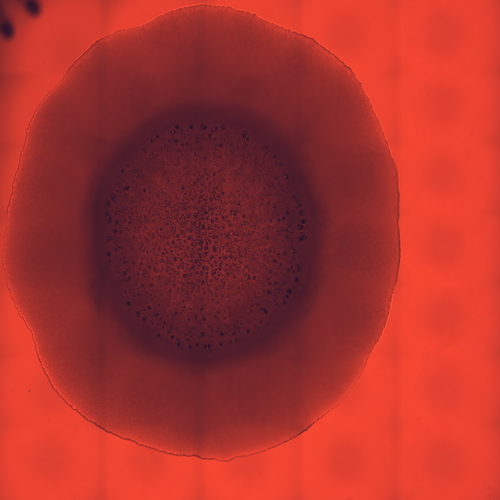
\includegraphics[width=4cm]{ResizedPIL-2_3dayLBCR-1.png}
\caption{A sample of Pseudomonas aeruginosa }
\label{FigResizedImage1}
\end{figure}



%=====METHODS=====
\section{Methods}
The methods used came from taking 10 random samples at a time  of Pseudomonas aeruginosa. Our samples had different tolerances to offset any biases in our results and model creation.


For the Linear Regression Model, we solved for beta with the following equation:

\begin{align}
\label{BetaEquation}
\bbeta \ = \ (\X^\T\X)^{-1}\X^\T\y.
\end{align}


Using the Linear Regression Equation:
\newline
\newline
    Linear Regression:
\begin{align}
\label{LinRegEq}
\y =\ \X\bbeta+\ep
\end{align}
\newline
 We got the following test results. 
\begin{figure}[h]
\centering
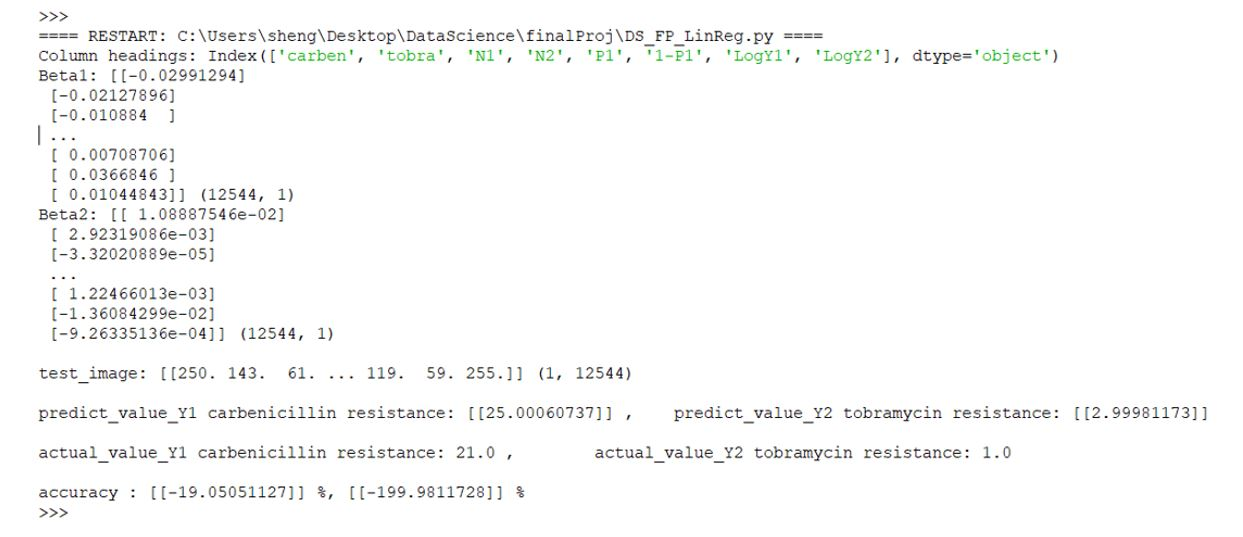
\includegraphics[width=8cm]{LinearReg_Result1}
\caption{Linear Regression Test Results}
\label{LinRegTestResult}
\end{figure}

The second method we used was logistic regression: We wanted to try another algorithm to classify our results and see how much more accurate of a prediction we could receive.
Logistic Regression:
\begin{align}
\label{LogRegEq}
p = \frac{1}{1+e^{-\beta^{T}x}}
\end{align}
\newline

After the Logistic Regression model was applied. The results indicates that ..see Figure \ref{LogRegTestResult}

\begin{figure}[h]
\centering
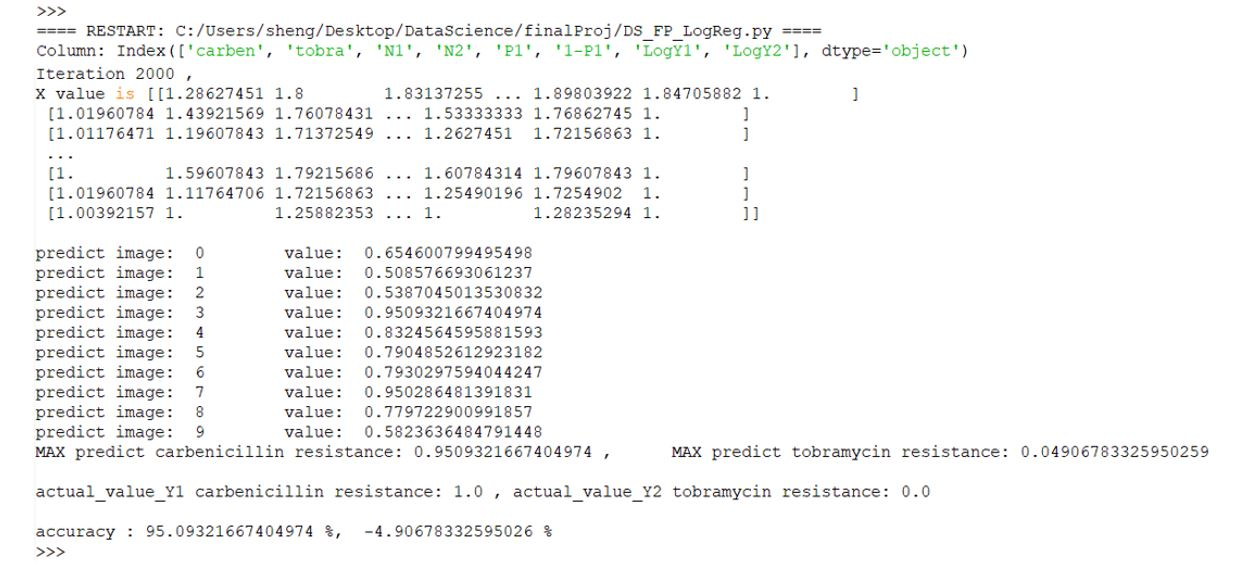
\includegraphics[width=8cm]{LogisticReg_Result1}
\caption{Logistic  Regression Test Results}
\label{LogRegTestResult}
\end{figure}


Then we used the Elbow Method mode,  \ref{ElboResult}l. The results indicates that six clusters should be appropriate in order to represent the data..

\begin{figure}[h]
\centering
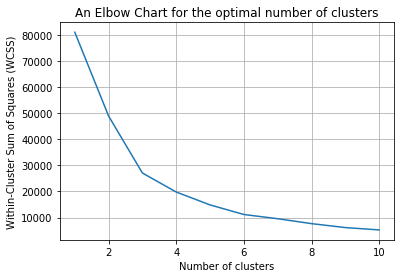
\includegraphics[width=8cm]{ElbowChart1.png}
\caption{Elbo Method  Result}
\label{ElboResult}
\end{figure}


Elbo Method model was applied. The results indecates that six clusters should be appropriate in order to represent the data. See figure 4.

We also used K-Means++ clustering algorithm to ascertain our findings. See figure \ref{KMeansResult}

\begin{figure}[h]
\centering
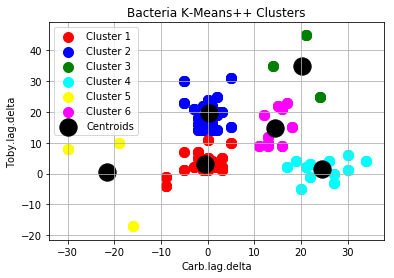
\includegraphics[width=8cm]{KMeansPP1.png}
\caption{KMeans++  Method  Test Result}
\label{KMeansResult}
\end{figure} 




%=====EXPERIMENTS=====
\section{Experiments}

There was a test image that we used to predict the values. Using our Linear Regression model, we get the values shown in \ref{tabLinearReg}.
\begin{table}[h]
\begin{center}
\begin{tabular}{| c || c | c |}
\hline
Image & Beta1(carben) & Beta2(tobra) \\ \hline \hline
1 & -0.02991294 & 1.08887546e-02 \\ \hline
2 & -0.02127896 & 2.92319086e-03 \\ \hline
\vdots & \vdots & \vdots \\ \hline
10 & 0.01044843 & -0.26335136e-04 \\ \hline
\end{tabular}
\caption{Linear Reg Results}
\label{tabLinearReg}
\end{center}
\end{table}

\begin{table}[h]
 Using our model we tested our models efficiency on our test image and got \ref{tabLinearRegResults}
\begin{center}
\begin{tabular}{| c || c | c |}
\hline
TestImage & Carbenicillin Resistance & Tobramycin \\ \hline \hline
Predicted & 25.00060737 & 2.99981173 \\ \hline
Actual & 21.0 & 1.0 \\ \hline
Accuracy & -19.05051127\% & -199.9811725\% \\ \hline
\end{tabular}
\caption{Linear Reg Results}
\label{tabLinearRegResults}
\end{center}
\end{table}

\begin{table}[h]
\begin{center}
\begin{tabular}{| c || c | c |}
\hline
Method & Antibiotic 1 & Antibiotic 2 \\ \hline \hline
Linear Regression & \textbf{0.12} & 0.18 \\ \hline
Logarithmic Regression & 0.16 & \textbf{0.13} \\ \hline
\end{tabular}
\caption{Predictions Mean Squared Error.}
\label{tabSummary}
\end{center}
\end{table}

Using the Logistic Regression Model we received the above Summarized Results \ref{tabSummary}.

%=====DISCUSSION=====
\section{Discussion}

Even though, we only fed ten pictures at a time to find its Beta value, our prediction on new image was quite accurate. Based on the experience we had from this project, if one needs to have a perfect model, it must meet several requirements. First, the picture needs quality with high resolution that allows every pixel to be distinguishable. This would help the accuracy improve. Second, computing power, when we computed, we resized the picture to 64x64 and it is float64, because some of the Python numpy libraries could not solve float32 with some matrix operations, that means one picture is 32768 bytes. So, 10x(64x64) was our training data size. Especially, when we performed dot product operation of Nx10 * 10xN, it takes at least 5 minutes just to finish one step. The best PC used was on 4.3Ghz processor and 16G RAM. Third, the logistic regression algorithm takes lots more time to find its pattern. During the maximum likelihood, we must run at 10 x (64x64) + 10 x (64x64) * learning steps which is unknown basing on the value of pixels. The Gradient Ascent is similar to the Restricted Boltzmann Machine we tried has very long-time training. One small error would have to start all over very time consuming.We tried to use a neural network to train our data to no avail, the code is provided.


%=====CONCLUSIONS=====
\section{Conclusion}
The linear regression algorithm was very good at determining the phenotype of the carbenicillin antibiotic resistance within 20\% accuracy. However, the accuracy of determining the tobramycin antibiotic resistance was much less accurate, missing the actual value by about 200\%.

The logistic regression algorithm overall was probably the better algorithm, the carbenicillin's resistance accuracy was about 95\% and the tobramycin's resistance was around 4\%.


%=====REFERENCES=====
\begin{thebibliography}{1}

\bibitem{paperName}
Sutskever, Ilya ,  Hinton, Geoffrey; and  Taylor, Graham.  \emph{The Recurrent Temporal Restricted Boltzmann Machine}, Advances in Neural Information Processing Systems 21, Proceedings of the Twenty-Second Annual Conference on Neural Information Processing Systems, Vancouver, British Columbia, Canada, December 8-11, 2008.


\end{thebibliography}

\end{document}


